\section{CNN의 구조와 장점}
\subsection{다층 CNN의 구조}
    CNN\footnote{Convolution Neural Network, 합성곱신경망} 알고리즘은 이미지를 대표할 수 있는 features(특성, 변수)를 이미지의 공간정보를 유지한채 추출하여 학습하는 알고리즘이다. 자율주행자동차, 얼굴인식과 같은 객체인식이나 computer vision이 필요한 분야에 많이 사용되고 있다. \\
    \vspace{-4mm}
    \begin{figure}[!h]\centering
		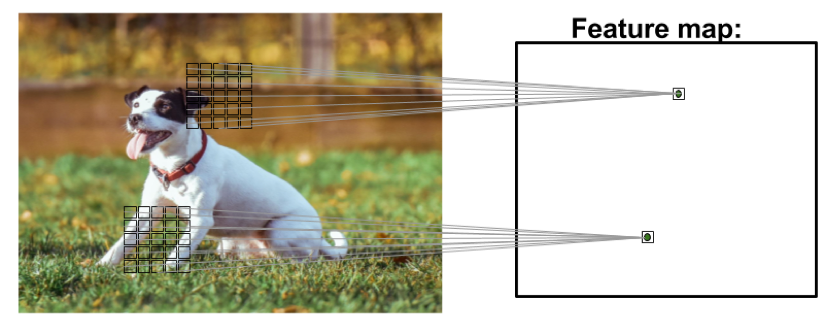
\includegraphics[width=.65\textwidth]{image/week04/2-1.png}
		\caption{\small Convolution Neural Network}
		\vspace{-10pt}
    \end{figure}
    
    CNN은 이미지의 특징을 추출하는 단계와 클래스를 분류하는 단계로 나뉜다. 특징 추출(Feature extraction/learning) 단계는 Convolution Layer와 Pooling Layer를 여러 겹 쌓는 형태로 구성된다. 
    CNN의 마지막에 위치한 이미지 분류(Classification) 단계에는 Fully Connected Layer가 있다. Flatten layer는 앞서 특징 추출 영역에서 추출한 이미지의 특징을 배열 형태로 나열한다. Softmax layer는 Fully Connected Layer를 거친 데이터를 바탕으로 Classification을 수행한다.
    \vspace{-4mm}
    \begin{figure}[!h]\centering
		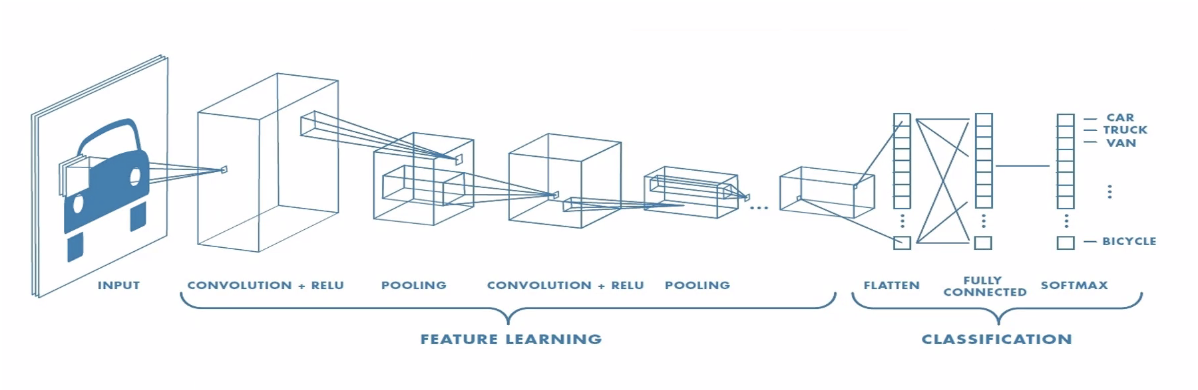
\includegraphics[width=.65\textwidth]{image/week04/2-2.png}
		\caption{\small CNN Structure}
		\vspace{-10pt}
    \end{figure}
    
    \subsubsection*{Convolution Layer}
    Convolution Layer는 이미지 분류(Classification)에 필요한 특징(feature)를 추출하는 layer이다. 하나의 Convolution Layer에는 하나의 filter가 존재한다. Filter는 아래의 그림과 같이 이미지 위를 차례대로 움직이면서 convolution(합성곱) 연산을 수행하여 합성곱 계층의 출력 이미지를 생성한다. 이미지의 각 영역에서 합성곱으로 도출된 값이 높을수록 filter에 부합하는 feature 정보라고 할 수 있다. CNN은 여러개의 filter를 사용하여 여러개의 feature를 추출한다. Filter 역시 초기 설정에는 무작위로 분포하지만 학습을 통해 자동으로 적절한 filter를 생성할 수 있다.
    \vspace{-4mm}
    \begin{figure}[!h]\centering
		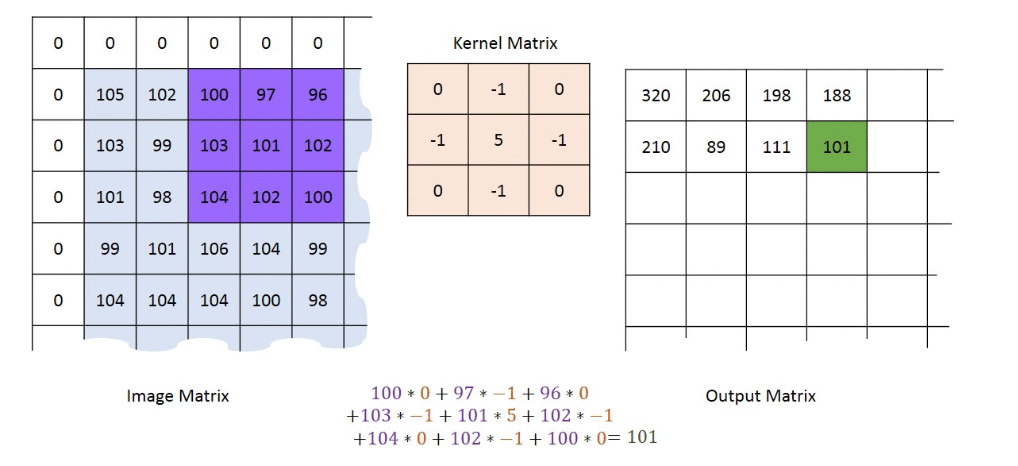
\includegraphics[width=.65\textwidth]{image/week04/2-3.png}
		\caption{\small Convolution Layer}
		\vspace{-10pt}
    \end{figure}
    
    \subsubsection*{Pooling Layer}
    원본 이미지 크기로 Fully Connected Layer로 가게 되면 연산량이 매우 클 것이다. Pooling Layer는 이미지의 크기를 줄이면서 특정 feature를 강조하는 역할을 한다. Pooling 방법에는 Max-pooling과 Mean-pooling이 있다. Max-pooling은 각 pooling 영역의 가장 큰 값을, Mean-pooling은 평균값을 대표값으로 선택한다. CNN은 주로 Max-pooling을 이용한다. 
    \vspace{-4mm}
    \begin{figure}[!h]\centering
		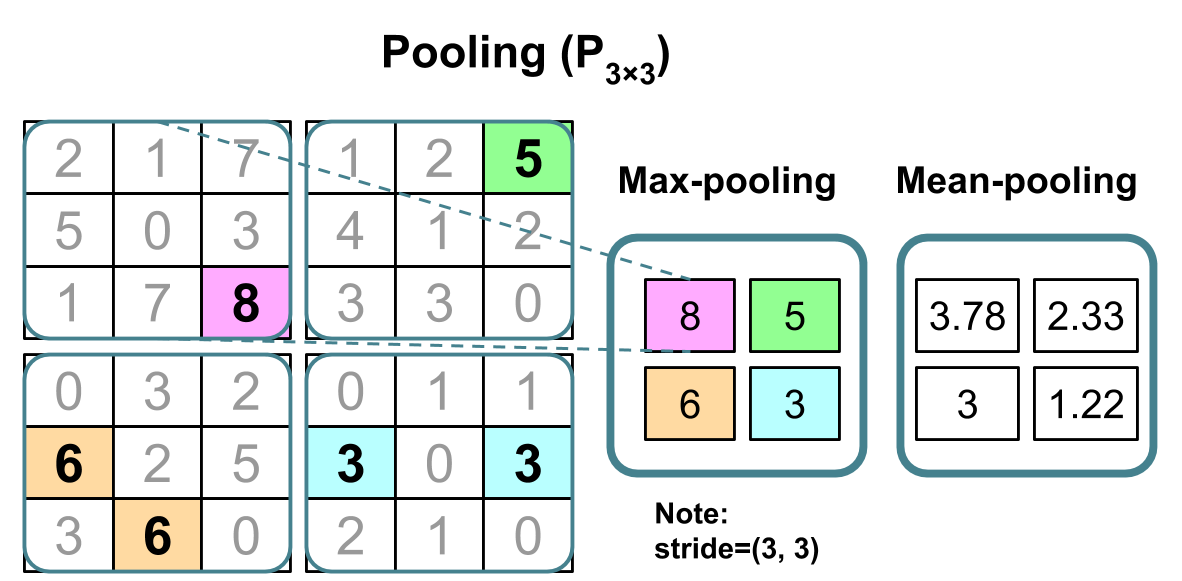
\includegraphics[width=.65\textwidth]{image/week04/2-4.png}
		\caption{\small Pooling Layer}
		\vspace{-10pt}
    \end{figure}
    
\subsection{CNN의 장점}
    CNN의 장점은 다음과 같다.
    \begin{enumerate}
        \item 적은 Parameter 수: FNN(Fully connected Neural Network)와 비교할때 parameter 수를 대폭 줄일 수 있기때문에 학습 시간을 줄이고 over fitting을 방지할 수 있다.
        \item Translation invariant: 다른 위치에서 동일한 feature를 추출할 수 있다.
        \item Locally connected: 이미지의 공간정보를 유지하면서 인접 이미지와의 위치적 특징을 효과적으로 인식할 수 있다.
    \end{enumerate}